% ICML 2026 AI for Good Workshop submission — clean rewrite (v3, 2026-05).
% Title: KWelfareBench: A Cell-Level Eligibility Benchmark and Conversational
%        Architecture for Korean Welfare Recommendation
% Camera-ready (accepted), ICML 2026 AI for Good Workshop.
% Compiles with the official ICML 2026 LaTeX style (icml2026.sty).

\documentclass{article}

\usepackage{microtype}
\usepackage{graphicx}
\usepackage{subcaption}
\usepackage{booktabs}
\usepackage{hyperref}
\newcommand{\theHalgorithm}{\arabic{algorithm}}

\usepackage[accepted]{icml2026}
\usepackage{amsmath}
\usepackage{amssymb}
\usepackage{mathtools}
\usepackage{amsthm}
\usepackage[capitalize,noabbrev]{cleveref}
\usepackage{url}
\usepackage{xcolor}
\usepackage{algorithm}
\usepackage{enumitem}
\usepackage{multirow}
\usepackage{float}

% ---- shorthand commands ----
\newcommand{\kwbench}{\textsc{KWelfareBench}}
\newcommand{\npolicy}{4{,}937}
\newcommand{\npersona}{180}
\newcommand{\nquery}{66}
\newcommand{\ndim}{69}

\icmltitlerunning{Closing the Welfare Outreach Gap}

\begin{document}

\twocolumn[
\icmltitle{Closing the Welfare Outreach Gap: \\
A Conversational Architecture and Cell-Level Eligibility Benchmark \\
for Korean Welfare Recommendation}

\icmlsetsymbol{cosecond}{$\dagger$}
\begin{icmlauthorlist}
\icmlauthor{Byeongmin Kang}{dgu}
\icmlauthor{Minwoo Han}{cosecond,inno}
\icmlauthor{Junhak Lee}{cosecond,raon}
\icmlauthor{Minsu Kim}{cosecond,inno}
\icmlauthor{Jihie Kim}{dgu}
\end{icmlauthorlist}
\icmlaffiliation{dgu}{Department of Computer Science and Artificial
Intelligence, Dongguk University, Seoul, Republic of Korea}
\icmlaffiliation{inno}{INNO-HI Inc., Republic of Korea}
\icmlaffiliation{raon}{RaonSecure Co., Ltd., Republic of Korea}
\icmlcorrespondingauthor{Jihie Kim}{jihie.kim@dgu.edu}
\icmlkeywords{AI for Good, conversational recommendation, welfare policy
recommendation, eligibility benchmark, Korean public sector, cell-level
evaluation, LLM-as-judge}

\vskip 0.3in
]
\printAffiliationsAndNotice{\textsuperscript{$\dagger$}These authors
contributed equally (co-second authors).}

% =====================================================================
\begin{abstract}
Welfare benefits often fail to reach the people who need them most,
including elderly citizens, digitally underserved users, and those
unfamiliar with eligibility categories, because portal-based search
requires users to know both \emph{which programs to search for} and
\emph{how their personal attributes map to eligibility criteria}.
This paper addresses the resulting outreach gap in three steps.
(1)~We propose a \emph{conversational welfare-policy recommendation
architecture} that elicits user attributes through natural-language
dialogue. (2)~To compare its core eligibility-matching component
quantitatively, we construct \emph{KWelfareBench}, a cell-level
eligibility ground-truth table over 4{,}937 Korean welfare policies
and 180 synthetic personas. (3)~Using this benchmark we compare
several recommendation architectures and identify an
eligibility-matching structure suited to the Korean welfare domain.
The resources, code, and personas are released as a shared
foundation for subsequent Korean welfare outreach research.
\end{abstract}

% =====================================================================
\section{Introduction}
\label{sec:intro}

\paragraph{The Korean welfare access problem.}
Korean welfare operates on an opt-in basis: a citizen must already
know that a relevant program exists, judge whether they qualify, and
submit an application before any benefit is delivered. The Korean
Ministry of Health and Welfare administers more than \npolicy{}
programs across central government, 17 \texttt{sido}, and 226
\texttt{sigungu}, and citizens are expected to query a keyword portal
under the assumption that they already know the program name, the
responsible agency, and the eligibility vocabulary. This excludes
precisely the populations whom welfare is intended to support:
digitally underserved older adults, low-income households, and
citizens combining several vulnerability axes.

\paragraph{Why current LLM/RAG systems are insufficient.}
Off-the-shelf RAG inherits four interacting weaknesses for
welfare: quantitative evaluation is
underdeveloped~\citep{kim_2024_govt_scheme_rag,alam_2024_sage_health};
generic retrievers ignore eligibility (a top-ranked policy can be
formally inapplicable); query pools leak persona attributes into
the surface form, confounding eligibility with intent; and
single-shot retrieval mismatches users who do not state every
relevant attribute up front.

\paragraph{Approach.}
We address these weaknesses through measurement. We separate
eligibility from intent into two independently labeled ground-truth
tables (GT-1, GT-2) and study their intersection (GT-3), the metric a
deployed assistant has to satisfy. The eligibility table is built
from a deterministic rule over a \ndim{}-binary $+$ 3-numeric tag
schema unified across policies and personas; the intent table is
graded $\{0,1,2\}$ by two independently prompted LLM judges with
cross-LLM agreement reported. A five-stage conversational loop closes
the back-end gap. The five stages are NL input (S1), tag extraction
(S2), query rewrite (S3), eligibility-aware retrieval (S4), and
follow-up question selection (S5); the loop is introduced fully in
\S\ref{sec:conv}, and only the recommendation and follow-up stages
(S4, S5) are evaluated end-to-end here, under oracle simulation of
the upstream NL stages (S1--S3).

\paragraph{Contributions.}
\textbf{(C1) \kwbench{}, a cell-level evaluation resource:} nine
release files covering \npolicy{} policies, \npersona{} synthetic
personas, a \ndim{}-binary tag schema, a 66-query persona-orthogonal
pool, and three ground-truth tables (GT-1 with 888{,}660 eligibility
cells, GT-2 with 325{,}842 graded intent cells, GT-3 the
intersection in six region/grading variants).
\textbf{(C2) Persona-orthogonal query taxonomy:} 33 sub-topics, two
phrasings each, curated under five rules R1--R5 so the query surface
is linearly independent of persona attributes; a multi-prefix
counterfactual rises from $8.7\%$ to $11.4\%$ non-zero topical
labels when persona prefixes are re-attached.
\textbf{(C3) Architecture comparison and conversational evaluation:}
six retrievers (B1--B6) on GT-2 and GT-3 (B2 ko-SBERT NDCG@10
$0.86$ on GT-2; B6 Rule\,+\,Dense $0.706$ on GT-3-strict;
\S\ref{sec:exp}), and a conversational back-end where a RandomForest
selector statistically matches exhaustive information-gain in
Recall@10 (turn-5 $0.095$ vs.\ $0.095$, n.s.) at ${\sim}1$\,ms per
turn---about $60\times$ less inference (\S\ref{sec:conv}). Reliability is validated
by a two-LLM full pass on A3 ($\kappa{=}0.822$) and A8
($\kappa_w{=}0.69$) with human adjudication of all disagreement
cells (\S\ref{sec:bench:reliability}). All artifacts are released
under KOGL Type~1 at
\url{https://github.com/choconaena/KWelfareBench}.

% =====================================================================
\section{Related Work}
\label{sec:related}

\paragraph{LLM-based recommenders and graded relevance.}
Modern recommender pipelines combine sparse retrievers
\citep{robertson2009bm25}, dense retrievers
\citep{karpukhin2020dpr,lewis2020rag}, and increasingly LLM rerankers
or end-to-end generative recommenders \citep{gao_2024_rag_survey}.
Evaluation typically follows the IR tradition of graded relevance
\citep{thakur2021beir}, expressing \emph{topical} relevance to a
query rather than whether a candidate is \emph{actionable} for a
specific user. In welfare recommendation the user is not implicit:
a topically relevant policy for which the user is statutorily
ineligible is a matching failure, yet existing benchmarks lack
the user-conditioned ground truth needed to measure this.

\paragraph{Public-sector and welfare AI.}
Public-sector welfare recommendation is a recently emerging area:
in 2024--2025 government-scheme matching tools
\citep{kim_2024_govt_scheme_rag}, small-government LLM applications
\citep{huggins_daines_2024_small_gov_llm}, homelessness and
social-security benefits chatbots
\citep{nelson2024llm_homelessness,hhs2024benefits_ai}, and
trust-and-ethics studies \citep{kaun_2025_public_sector_chatbots}
have appeared. Together they demonstrate feasibility but typically
evaluate top-$K$ accuracy on a small demonstration persona set, do
not release a reusable ground-truth table, and are not directly
comparable across architectures. Per-segment fairness diagnostics
follow the intersectional framework of \citet{wang_2024_itfr_www}.

\paragraph{Korean policy retrieval and LLM-as-judge.}
Empirical work on Korean welfare retrieval is minimal: the
\emph{Bokjiro} portal exposes only a keyword interface; general
government-scheme RAG prototypes \citep{kim_2024_govt_scheme_rag}
demonstrate feasibility but release no reusable ground-truth table;
and \citet{ban2025welfare_disabled} focuses on a single
sub-population.
The closest non-welfare analogue is TrialGPT
\citep{jin_2024_trialgpt} for clinical-trial eligibility, whose
cell-level patient--trial structure is structurally identical to a
persona--policy table but assumes users already know their
attributes. Recent personalized LLM-assistant benchmarks
\citep{liu2025personalens} share the cell-level philosophy.
Constraint-based recommendation
\citep{jannach_2015_constraint_recsys,felfernig_2023_rdf_constraint_rec}
provides a complementary lens, hard rules over user attributes,
which we instantiate as our rule eligibility function. LLM-as-judge
labeling is now common
\citep{zheng2023mtbench,judges_verdict2025}; we cross-validate two
independently prompted judges and report quadratic-weighted
$\kappa$ \citep{cohen1968weightedkappa} appropriate for ordinal
$\{0,1,2\}$ labels. \citet{andukuri2024clarinet} learns a
retrieval-aware clarification policy end-to-end; our selector is a
simpler RandomForest whose advantage is sub-millisecond inference.

% =====================================================================
\section{\kwbench{}}
\label{sec:benchmark}

\subsection{Overview: Released Resource Catalogue}
\label{sec:bench:overview}

\kwbench{} ships as nine release artifacts (A1--A9,
Table~\ref{tab:bench_artifacts}) that fall into three groups:
(i) raw policy data and regional standard labels (A1--A2,
\S\ref{sec:bench:a1}--\S\ref{sec:bench:a2}); (ii) the unified tag
schema and the persona corpus, with both sides labeled in the same
schema (A3--A5, \S\ref{sec:bench:a3}--\S\ref{sec:bench:a5}); (iii) the
persona-orthogonal query pool (A6, \S\ref{sec:bench:a6}) and the
three ground-truth tables with six derived matrices (A7--A9,
\S\ref{sec:bench:a7}). Reliability of the LLM labels underlying A3 and
A8 is reported in \S\ref{sec:bench:reliability}. The pipeline is
summarised in Figure~\ref{fig:overview}.

\begin{figure}[t]
\centering
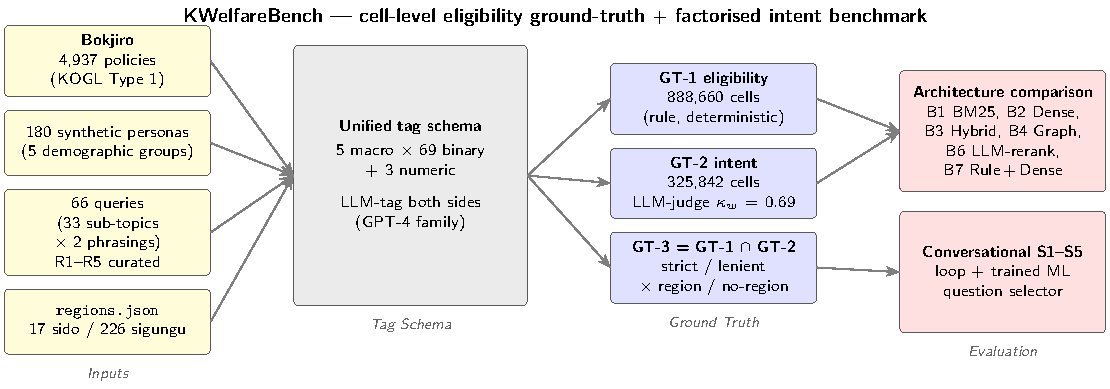
\includegraphics[width=\columnwidth]{figures/fig1_overview.pdf}
\caption{\kwbench{} pipeline overview. Raw policies (A1) and the
regional standard (A2) feed a unified tag schema (A3, A5) shared with
the synthetic persona corpus (A4); the persona-orthogonal query pool
(A6) and the three ground-truth tables (A7 GT-1 eligibility, A8 GT-2
intent, A9 GT-3 intersection) drive the architecture comparison
(\S\ref{sec:exp}) and the conversational evaluation
(\S\ref{sec:conv}).}
\label{fig:overview}
\end{figure}

\begin{table}[t]
\centering
\footnotesize
\setlength{\tabcolsep}{4pt}
\begin{tabular}{llll}
\toprule
ID & Artifact & Format & Size \\
\midrule
A1 & Raw policies         & JSON & \npolicy{} policies \\
A2 & Regional standard    & JSON & 17 sido / 226 sigungu \\
A3 & Policy tags          & JSON & \npolicy{}\,$\times$\,72 \\
A4 & Synthetic personas   & JSON & \npersona{} personas \\
A5 & Persona tags         & JSON & \npersona{}\,$\times$\,72 \\
A6 & Query pool           & JSON & 33 topics, 66 queries \\
A7 & GT-1 eligibility     & NPZ  & 888{,}660 cells \\
A8 & GT-2 intent (graded) & NPZ  & 325{,}842 cells \\
A9 & GT-3 intersection    & NPZ  & $11{,}880\!\times\!3$ \\
\bottomrule
\end{tabular}
\caption{The nine \kwbench{} release artifacts. All files are
released under KOGL Type~1, the same licence as the Bokjiro source.
A9 ships in three region variants ($\times{}3$: strict, sido-only
lenient, region-agnostic) crossed with two grading thresholds,
yielding the six derived GT-3 matrices.}
\label{tab:bench_artifacts}
\end{table}

\subsection{A1--A2: Raw Snapshot and Regional Standard}
\label{sec:bench:a1}
\label{sec:bench:a2}

\textbf{A1.} Policy metadata from \emph{Bokjiro}
(\url{https://www.bokjiro.go.kr}), the Korean Ministry of Health and
Welfare's portal. As of an April~2026 snapshot, the collection
contains \npolicy{} programs (name, summary, description, eligibility
text, benefits, application procedure, region, responsible agency).
The Bokjiro footer (accessed 2026-04) states ``Gonggongnuri Type~1
(KOGL)''---attribution required, commercial use allowed, modification
allowed; all A1--A9 inherit this licence.
\textbf{A2.} A frozen list of 17 \texttt{sido} and 226
\texttt{sigungu}, released alongside the tag schema. The eligibility
function in \S\ref{sec:bench:a7} consumes these standard codes;
free-text neighborhood preferences live in a separate
\texttt{region.nl} channel and surface only at the GT-2 retrieval
layer.

\subsection{A3: Policy Tag Labels (\ndim{} binary $+$ 3 numeric)}
\label{sec:bench:a3}

We design a hierarchical schema of five macro-categories
(PERSONAL, ECONOMIC, HOUSEHOLD, SOCIAL, POLICY) over \ndim{} binary
tags (Figure~\ref{fig:schema}; full list in
Appendix~\ref{app:schema}). The first four follow the standard
four-axis eligibility taxonomy used in Korean social-welfare
textbooks; POLICY (welfare, employment, education, housing, health,
culture, living) takes the seven category labels used in Bokjiro's
policy-classification metadata field, which is distinct from the
fifteen search-filter sub-topics exposed in Bokjiro's public UI. We
verified that all \npolicy{} policies in our snapshot carry one of
these seven labels.
Each binary tag takes one of three values:
$+1$ \emph{required}, $-1$ \emph{excluded} (disqualifies the
applicant), or $0$ \emph{indifferent}. The 3-state representation
distinguishes ``not mentioned'' from ``explicitly excluded'',
which noticeably affects matching precision. Three numeric fields
(\texttt{age\_min}, \texttt{age\_max},
\texttt{median\_threshold}) complete the schema.

\begin{figure}[t]
\centering
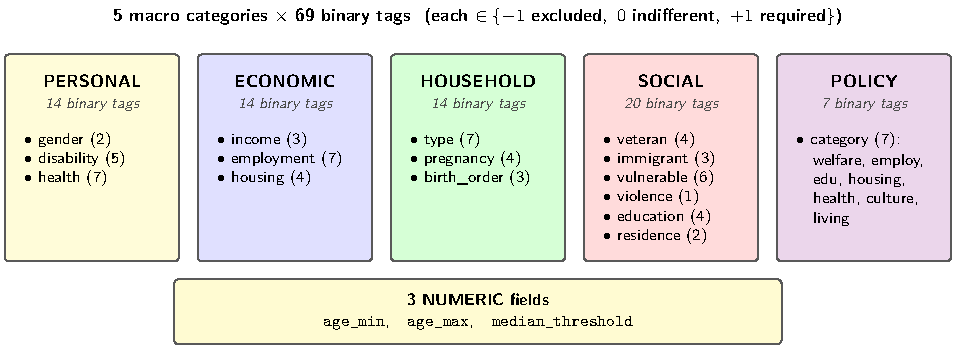
\includegraphics[width=\columnwidth]{figures/fig2_schema.pdf}
\caption{The \kwbench{} tag schema: 5 macro-categories
$\times$ \ndim{} binary tags $+$ 3 numeric fields. PERSONAL,
ECONOMIC, HOUSEHOLD, and SOCIAL describe \emph{eligibility} (shared
between policies and personas); POLICY describes \emph{program type}
and inherits the seven Bokjiro categories.}
\label{fig:schema}
\end{figure}

\paragraph{Construction.}
We call \texttt{gpt-5.4} (OpenAI chat-completions API; April~2026;
temperature~0) in parallel: each prompt includes the policy's name,
summary, eligibility text, benefits, application procedure, and
region, and the model emits the $\ndim{}+3=72$ values on a single
comma-separated line rather than as JSON. The comma-separated form
reduces output tokens by roughly $5.5{\times}$ (per-policy cost and
total runtime details in Appendix~\ref{app:repro}). Reliability is
reported in \S\ref{sec:bench:reliability}.

\subsection{A4--A5: Personas and Persona Tag Labels}
\label{sec:bench:a4}
\label{sec:bench:a5}

The \npersona{} personas (A4) are organized as
\textbf{Base (50)}, ten personas in each of five reference groups
(disability, single parent, senior, youth, general);
\textbf{Extra (80)}, regional coverage spanning 17 provinces and
226 districts; and \textbf{Intersectional (50)}, 18 intersectional
axes with 1--6 personas each. The five reference groups span the
at-risk groupings most frequently cited in MOHW yearbooks and
represented by Bokjiro's recommendation filter; the alignment is not
one-to-one (Bokjiro's filter additionally distinguishes
multi-cultural and multi-child families, which we fold into
intersectional axes rather than top-level groups). Each persona is
synthesized with stratified sampling (gender 50/50, group-specific
age, 17-sido weighted distribution); the seed and the generator are
released, and all personas are synthetic with no PII.

\textbf{A5.} Each persona's attributes are encoded as
\texttt{tag\_values} that mirror the policy-side \ndim{}-binary
$+$~3-numeric schema, so the eligibility function runs on a single
shared vocabulary across both sides of the cell-level table.

\textbf{Sample-size design.} We chose $n{=}\npersona{}$
($5$ groups $\times$ $36$) to keep $\geq{}30$ per group for
stratified bootstrap CIs while keeping the LLM tagging budget
feasible; the L5 limitation discusses scale-up.

\subsection{A6: Persona-Orthogonal Query Pool}
\label{sec:bench:a6}

To evaluate retrieval that respects \emph{user intent} (GT-2)---i.e.,
topical relevance between a free-form query and a candidate---we
construct a pool of \textbf{\nquery{} queries} drawn from
\textbf{33 sub-topics}, paired with each \npersona{} persona at test
time. The central design requirement is
\emph{persona-orthogonality}: the sub-topic taxonomy is
linearly independent of the 9-dimensional persona attribute space
used by the eligibility function. If a sub-topic embeds a token like
``youth'' or ``low-income'', GT-1 and GT-2 confound and retrieval
failures cannot be attributed to mismatched eligibility vs.\ intent.

\textbf{Stage 1.} We adopt the seven Bokjiro macro-categories
(welfare, employment, education, housing, health, culture, living)
as the top of the taxonomy. From each we randomly sample 30 policies
and prompt \texttt{gpt-5.4-mini} (temperature~0) to extract
candidate sub-topics under the \emph{interest unit} criterion;
98 raw candidates result.
\textbf{Stage 2 (curation, five rules).} Two authors independently
apply: \textbf{(R1) Persona-orthogonality}, reject sub-topics whose
surface form mirrors a persona attribute (``youth rent assistance''
$\to$ ``rent assistance''); \textbf{(R2) Topical consolidation},
merge same-concern sub-topics (\{school-uniform, child-care, loans,
scholarships\} $\to$ \emph{tuition and education-cost support});
\textbf{(R3) Coverage granularity}, each sub-topic must match
$\geq{}30$ policies (mean $>{}100$);
\textbf{(R4) Cross-category deduplication}, one best-fit category
each; and \textbf{(R5) No specific values} (no region names, exact
ages, income amounts). The 98 raw sub-topics reduce to 33 (welfare
5, employment 4, education 4, housing 5, health 5, culture 4, living
6). \textbf{Stage 3 (phrasing).} Two query variants per sub-topic, a
\emph{procedural} (``how do I apply for X support?'') and a
\emph{situational} (``X is becoming financially hard for me\ldots''),
yielding $33{\times}2 = \nquery{}$ queries, each 10--25 Korean
characters.

\paragraph{R1-violation ablation.}
To check that R1 actually matters, we re-prepend ten representative
demographic prefixes (senior, disabled, single-parent, youth,
multi-child, multicultural, newlywed, low-income, pregnant,
basic-recipient) to the sub-topics and re-grade a stratified
$4{,}950$-cell sample with the independent judge
\texttt{gemini-2.5-flash-lite}.\footnote{We use an LLM judge
rather than a semantic-similarity classifier because the question
is whether a re-prefixed query \emph{changes the
recommendation-relevant intent} of the cell, which requires
welfare-policy domain knowledge a similarity classifier lacks; on
this subset the OpenAI judge agrees at $\kappa_w{=}0.71$.}
Pooled across the ten prefixes, the fraction
of non-zero (graded $\geq{}1$) labels rises from $8.7\%$ to
$11.4\%$ ($\Delta{=}{+}2.6$\,pp); 8 of 10 prefixes show positive
shifts, full distribution in Figure~\ref{fig:r1-multiprefix}. The
direction supports R1: re-attaching demographics inflates topical
relevance, which is exactly the leak factoring eligibility from
intent is meant to prevent.

\begin{figure}[t]
\centering
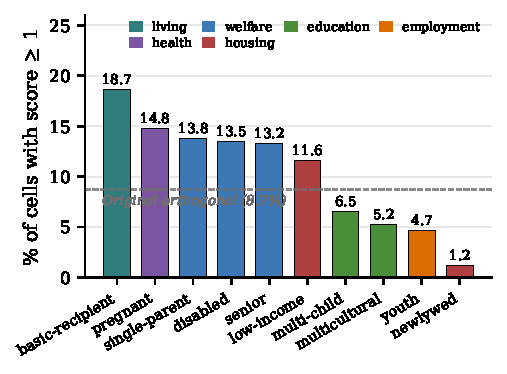
\includegraphics[width=\columnwidth]{figures/fig8_r1_multiprefix.pdf}
\caption{R1-violation multi-prefix ablation: \% of cells scoring
$\geq 1$ when the persona-orthogonal query is prefixed by 10
demographic identifiers. Pooled mean $11.4\%$ vs.\ orthogonal
baseline $8.7\%$ ($+2.6$pp). The variance across prefixes
(1.2\% newlywed $\to$ 18.7\% basic-recipient) shows R1 violations
have heterogeneous semantic spillover.}
\label{fig:r1-multiprefix}
\end{figure}

\subsection{A7--A9: Three Ground-Truth Tables}
\label{sec:bench:a7}

\textbf{GT-1 (A7) rule-based eligibility.}
A deterministic function
$\mathrm{eligible}(\pi,p)\in\{0,1\}$ requires \emph{all} nine
dimensions (logical AND): income, special, age, gender, employment,
household, education, sigungu, sido. Separating the dimensions
allows attribution of failures during diagnostic analysis. Region
matching uses only A2 codes; free-text \texttt{region.nl} preferences
are deferred to GT-2. A citizen is rule-eligible for
$\approx{}1.96\%$ of all programs (mean $97.0$ per persona; group
breakdown in Table~\ref{tab:group_stats}).
\textbf{GT-2 (A8) graded intent.}
For each (query, policy) pair we elicit a 3-point label
($0$ unrelated, $1$ adjacent, $2$ direct) from
\texttt{gpt-5.4-nano} (primary) and
\texttt{gemini-2.5-flash-lite} (cross-vendor), each prompted
independently with a shared few-shot anchor set, over
$\nquery{}\times\npolicy{}=325{,}842$ cells per judge.
\textbf{GT-3 (A9) intersection.}
A policy is in GT-3 when both GT-1-eligible \emph{and} GT-2-relevant.
We release six matrices: $\{$strict ($=2$), lenient
($\geq{}1$)$\}$ grading $\times$ $\{$strict, lenient, no-region$\}$
region. \textbf{GT-3-strict} (mean $\bar n_{\mathrm{el}}{=}4$
targets per pair, $20.86\%$ empty cells) is the operating point a
deployed assistant has to clear.

\paragraph{Group-level eligibility counts.}
Vulnerable groups are eligible for more policies than the general
population (Table~\ref{tab:group_stats}: disability $122$ vs.\
general $73$, $+{}67\%$), reflecting the program-side volume
targeted at these groups---distinct from the \emph{application
rate} behind the opt-in outreach gap.

\begin{table}[t]
\centering\small
\begin{tabular}{lrr}
\toprule
Persona group & $n$ & Mean eligible policies \\
\midrule
Disability      & 26 & \textbf{122.2} \\
Senior          & 28 & 108.4 \\
Intersectional  & 50 & 103.5 \\
Single parent   & 24 & 89.2 \\
Youth           & 26 & 78.2 \\
General         & 26 & 73.0 \\
\midrule
\textbf{Total}  & \textbf{180} & \textbf{97.0} \\
\bottomrule
\end{tabular}
\caption{\kwbench{} mean eligible-policy count by persona group.}
\label{tab:group_stats}
\end{table}

\subsection{Reliability: Cross-LLM and Human Audit}
\label{sec:bench:reliability}

Every LLM-judged release artifact (A3, A8) follows the same
two-LLM-full-pass plus human-on-disagreement protocol. The human
adjudicators have welfare-policy backgrounds (graduate-student
researchers and domain practitioners), treated as a strong
reliability tier above pure LLM labels but below a
credentialed-expert audit (\S\ref{sec:limit}, L6).

\textbf{A3 (policy tags).} Both \texttt{gpt-5.4} and
\texttt{gpt-5.5} independently emitted the full
$\npolicy{}\times{}72$ tag matrix at temperature~0. The two LLMs
agree on $\mathbf{96.8\%}$ of the $\sim{}356{,}000$ binary cells
($\kappa{=}0.822$, ``almost perfect''). Numeric-field agreement is
high (\texttt{age\_min} $98\%$, \texttt{age\_max} $96\%$,
\texttt{median\_threshold} $100\%$). The LLM-disagreement set
($n{\approx}11{,}400$ cells, $3.2\%$) was split four ways and
fully adjudicated by the reviewer team in a 30-minute consensus
pass per shard. The released A3 uses human adjudication on the
disagreement set and the LLM-majority label on the agreement set.

\textbf{A8 (query--policy intent).} Both \texttt{gpt-5.4-nano} and
\texttt{gemini-2.5-flash-lite} graded all $325{,}842$ cells
independently with a shared few-shot anchor set. Cross-LLM
agreement is $\mathbf{91.03\%}$ ($\kappa_{\mathrm{unweighted}}{=}0.50$,
$\kappa_w{=}0.69$~\citep{cohen1968weightedkappa}); disagreements
concentrate on adjacent grades. The agreement set
($n{=}296{,}575$) was sanity-checked with a 100-cell uniform
random sample reviewed independently by four humans, who concurred
with the LLM majority on $\mathbf{96/100}$ cells (the four
disagreements were single-step $1\!\leftrightarrow\!2$). The
disagreement set ($n{=}29{,}267$, $8.97\%$) was split four ways and
fully adjudicated. The released A8 uses human adjudication on the
disagreement set and the LLM-majority label on the agreement set;
\texttt{gpt-5.4-nano} is the primary alias for downstream metrics.

% =====================================================================
\section{Architecture Comparison}
\label{sec:exp}

\subsection{Setup}
\label{sec:exp:setup}

\paragraph{Task and metrics.}
Given a persona's natural-language query, return the top-$K$
candidate policies among the \npolicy{} \kwbench{} programs.
Evaluation metrics, computed against \kwbench{} ground truth, are
Precision@$K$, Recall@$K$, and NDCG@10 for $K\in\{5,10,20\}$, with
$K{=}10$ used as the primary cutoff throughout. Means are
reported with bootstrap $95\%$ CIs ($N_{\mathrm{boot}}{=}10{,}000$,
query-level resampling); pairwise comparisons use the paired Wilcoxon
signed-rank test \citep{wilcoxon1945signed} with Holm--Bonferroni
correction \citep{holm1979bonferroni}.

\paragraph{Components.}
BM25Okapi \citep{robertson2009bm25,trotman2014bm25vskl}
($k_1{=}1.5,b{=}0.75$); dense retriever
\texttt{jhgan/ko-sroberta-multitask} \citep{park2023kosroberta,reimers2019sbert}
(768-d Korean SBERT, KorNLI/KorSTS contrastive); RRF
($k_{\mathrm{RRF}}{=}60$) \citep{cormack2009rrf}; LLM rerank judges
\texttt{gpt-5.4-nano} and \texttt{gemini-2.5-flash-lite}.
Policy text concatenates \texttt{name$\Vert$summary$\Vert$
eligibility$\Vert$benefits} (mean 247 Korean characters); no
chunking. BM25 uses a hybrid Hangul tokenizer (whitespace $+$ 2-gram
syllable backoff).

\paragraph{Baselines.}
\textbf{B1 BM25}; \textbf{B2 Dense} (ko-SBERT) with multilingual
variant \textbf{B2$^\prime$ BGE-M3} (BAAI/bge-m3 single-vector dense);
\textbf{B3 Hybrid} (RRF of B1 \& B2);
\textbf{B4 Graph} (cosine of persona-satisfied vs.\ policy-required
tag sets, Appendix~B.4);
\textbf{B5 LLM-rerank} (BM25 top-50 reranked by Gemini with
structured-output enforcement) with cross-encoder variant
\textbf{B5$^\prime$ BGE-reranker-v2-m3} (BAAI multilingual
cross-encoder reranking BM25 top-200);
\textbf{B6 Rule $+$ Dense rerank} (rule prefilter then ko-SBERT
rerank). Matched-prefilter controls \textbf{B2$+$rule} and
\textbf{B5$+$rule} apply the rule prefilter then rerank by Dense or
Gemini; B6 $=$ B2$+$rule by construction. We omit a rule-only
competitor on GT-3: it shares the predicate with the ground truth
and would be circular.

\subsection{GT-2 Results: Intent-Only Retrieval}
\label{sec:exp:gt2}

GT-2 is computed on the $\nquery{}\times\npolicy{}{=}325{,}842$
query--policy cells with graded LLM-judge labels and is
persona-independent. Table~\ref{tab:gt2} reports NDCG@10, P@10
(graded $\geq{}2$), and R@10 (graded $\geq{}2$) for the four
\emph{rule-free} retrievers; B4 (Graph) and B6 (Rule$+$Dense) are
inherently persona-conditioned and therefore have no natural
query-only formulation, so the GT-2 column for them is omitted by
design.

\begin{table}[t]
\centering\scriptsize
\setlength{\tabcolsep}{3pt}
\begin{tabular}{lrrr}
\toprule
Baseline & NDCG@10 & P@10$_{\geq 2}$ & R@10$_{\geq 2}$ \\
\midrule
\multicolumn{4}{l}{\emph{Sparse / lexical}} \\
B1 BM25-Okapi & 0.642 & 0.544 & 0.096 \\
\midrule
\multicolumn{4}{l}{\emph{Dense (single-vector cosine)}} \\
B2 ko-SRoBERTa            & \textbf{0.858}$^*$ & \textbf{0.752}$^*$ & \textbf{0.142}$^*$ \\
B2$^\prime$ BGE-M3        & 0.815 & 0.698 & 0.126 \\
\midrule
\multicolumn{4}{l}{\emph{Cross-encoder rerank (BM25 top-200)}} \\
B5$^\prime$ BGE-reranker-v2-m3   & 0.853 & 0.752 & 0.139 \\
\midrule
\multicolumn{4}{l}{\emph{Hybrid / LLM-rerank}} \\
B3 Hybrid (RRF, B1$+$B2)  & 0.849 & 0.745 & 0.134 \\
B5 Gemini-rerank (BM25 top-50)   & 0.789 & 0.683 & 0.126 \\
\bottomrule
\end{tabular}
\caption{GT-2 (intent-only) retrieval over the 66 queries $\times$
\npolicy{} policies. Bootstrap $95\%$ CIs (query-level resampling,
$N_{\mathrm{boot}}{=}10{,}000$): B2 NDCG@10 $[0.81, 0.90]$, B1 NDCG@10
$[0.57, 0.71]$. $^*$Dense (B2 ko-SRoBERTa) $>$ BM25 paired Wilcoxon
$p{<}10^{-8}$; Hybrid vs.\ Dense is not statistically distinguishable
on NDCG@10 ($p{=}0.76$). The cross-encoder reranker
BGE-reranker-v2-m3 (BAAI multilingual) reranks BM25 top-200; the
multilingual BGE-M3 embedding (BAAI/bge-m3) replaces ko-SRoBERTa as
a single-vector dense retriever. An auxiliary Korean cross-encoder
result (\texttt{ko-reranker}) is reported in
Appendix~\ref{app:auxiliary}.}
\label{tab:gt2}
\end{table}

\begin{figure}[t]
\centering
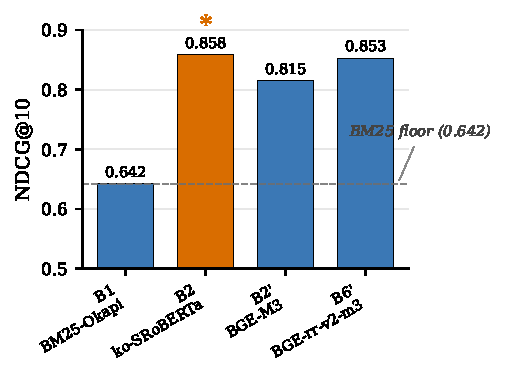
\includegraphics[width=\columnwidth]{figures/fig6_gt2_baselines.pdf}
\caption{GT-2 (graded) NDCG@10 across baselines. ko-SRoBERTa (B2)
and BGE-reranker-v2-m3 (B5$^\prime$) tie at the top; the
multilingual BGE-M3 underperforms on the persona-orthogonal query
distribution. Dashed line: BM25 floor.}
\label{fig:gt2-baselines}
\end{figure}

\paragraph{Finding 1.}
Korean-text dense retrieval (B2 ko-SRoBERTa) is the strongest
rule-free retriever on GT-2 by a small but consistent margin
(Figure~\ref{fig:gt2-baselines}). We were initially surprised that
the multilingual BGE-M3 underperforms the Korean ko-SRoBERTa given
that domain mismatch usually runs the other way; we attribute this
to the persona-orthogonal queries staying close to Bokjiro's own
phrasing, where Korean-specific contrastive pretraining pays off.
Two cross-encoder rerankers further support the finding:
(i)~the multilingual BGE-M3 single-vector embedding scores $-0.04$
NDCG@10 below ko-SRoBERTa ($0.815$ vs.\ $0.858$), suggesting that a
Korean-specific embedding remains preferable to multilingual SOTA
on this corpus; (ii)~the multilingual cross-encoder
BGE-reranker-v2-m3, applied as a rerank over BM25 top-200, attains
$0.853$ NDCG@10, within $0.005$ of the Korean dense backbone but
roughly $190\times$ slower per query (\S\ref{sec:exp:latency}). The
hybrid (B3) does not improve over ko-SRoBERTa alone, so BM25 noise
appears to hurt rather than help when fused. The Gemini LLM-rerank
(B5) lifts BM25 from $0.642$ to $0.789$ NDCG@10 yet remains below
B2.

\subsection{GT-3 Results: Eligibility$\,\cap\,$Intent}
\label{sec:exp:gt3}

GT-3 is the metric a deployed assistant has to satisfy: a returned
policy must be \emph{both} eligible for the persona \emph{and}
topically relevant to the query.
Table~\ref{tab:gt3} reports the strict variant (graded $=2$, strict
region match; $\bar n_{\mathrm{eligible}}{=}4$) over $11{,}880$
(persona, query) pairs; the lenient variant follows the same
ordering. Figure~\ref{fig:gt2gt3} visualises both panels jointly.

\begin{table}[t]
\centering\small
\setlength{\tabcolsep}{4pt}
\begin{tabular}{lrrr}
\toprule
Baseline & NDCG@10 & P@10 & R@10 \\
\midrule
\multicolumn{4}{l}{\emph{Rule-free}} \\
B1 BM25      & 0.071 & 0.027 & 0.092 \\
B2 Dense     & 0.119 & 0.051 & 0.133 \\
B3 Hybrid    & 0.102 & 0.042 & 0.135 \\
B4 Graph     & 0.122 & 0.047 & 0.126 \\
\midrule
\multicolumn{4}{l}{\emph{Rule-augmented (matched prefilter)}} \\
B5$+$rule    & 0.249 & 0.073 & 0.208 \\
B6 (B2$+$rule) & \textbf{0.706} & \textbf{0.341} & \textbf{0.742} \\
\bottomrule
\end{tabular}
\caption{GT-3 strict (eligibility $\cap$ intent, strict region match).
$11{,}880$ (persona, query) pairs. \textbf{B5$+$rule} denotes B5
(Gemini-rerank) applied after the rule prefilter, the matched-control
counterpart of B6 (Dense rerank after the same prefilter). B5$+$rule
and B6 share the \emph{same} rule prefilter; the only difference is
the rerank function (Gemini vs.\ Dense). Holding the prefilter
constant, Dense rerank dominates Gemini rerank by $+0.46$ NDCG@10.
Lenient-grading counterpart: B6 NDCG@10 $0.697$, B5$+$rule $0.162$.}
\label{tab:gt3}
\end{table}

\begin{figure}[t]
\centering
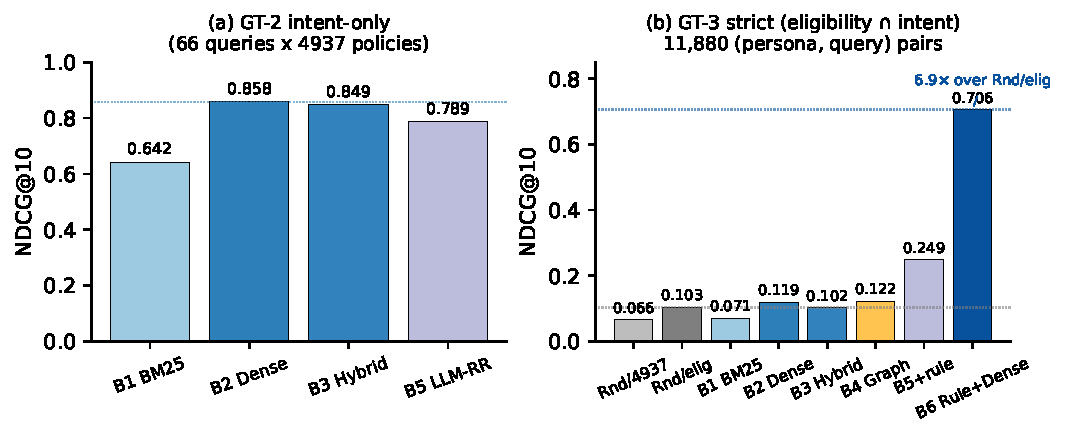
\includegraphics[width=\columnwidth]{figures/fig3_gt2_gt3_comparison.pdf}
\caption{NDCG@10 across architectures on (a) GT-2 intent-only
retrieval over $325{,}842$ cells and (b) GT-3 strict
(eligibility$\cap$intent) over $11{,}880$ (persona, query) pairs.
B4 (Graph) and B6 (Rule$+$Dense) are persona-conditioned and
therefore omitted from (a). In (b), the two leftmost gray bars are
random baselines --- uniform random over all $4{,}937$ policies
($0.066$) and over the rule-eligible subset ($0.103$). B6 attains a
$\approx{}6.9{\times}$ lift over the rule-conditioned chance level;
B5$+$rule and B6 share the same rule prefilter, so the gap between
them directly isolates the rerank-method contribution.}
\label{fig:gt2gt3}
\end{figure}

\paragraph{Finding 2.}
Without a rule prefilter, every rule-free retriever collapses to
NDCG@10 around $0.12$ on GT-3-strict (B1--B4 in $[0.07, 0.13]$), an
order of magnitude below GT-2. Topical relevance alone is
insufficient when eligibility is the gate.

\paragraph{Finding 3 (matched-prefilter diagnostic).}
B5$+$rule and B6 differ only in the rerank function (Gemini vs.\
Dense) atop an identical rule prefilter. Dense rerank dominates by
$+0.46$ NDCG@10, so the rerank \emph{ordering} contributes
substantively over and above the prefilter; the operationally best
recipe on GT-3 is rule-eligibility prefilter $+$ Korean-domain dense
rerank.

\paragraph{Sparsity caveat and random baselines.}
GT-3-strict is intrinsically sparse: $\bar n_{\mathrm{el}}{=}4$
targets per (persona, query) pair and $20.86\%$ of cells are empty
(no policy is both rule-eligible and graded $=2$). To confirm the
absolute level of B6's NDCG@10$=0.706$ is meaningful rather than an
artifact of sparse target sets, we compare against two random
baselines under the same metric. (i) Uniform random over all
\npolicy{} policies yields NDCG@10$\approx{}0.066$, the chance level
when no signal is used at all. (ii) Uniform random over the
rule-eligible subset (mean 97 candidates per persona) yields
NDCG@10$\approx{}0.103$, the chance level conditional on the
eligibility prefilter alone. B6's $0.706$ is $\approx{}6.9\times$
above this rule-conditioned chance level, confirming that the dense
rerank ordering carries substantive signal beyond what the
eligibility prefilter contributes by itself, and that the rule$+$dense
gap over B5$+$rule (Finding~3) is not a sparsity artifact
(Figure~\ref{fig:gt2gt3}(b), where the two random baselines are shown
as gray bars to the left of the architecture comparison).

\subsection{Latency and Statistical Tests}
\label{sec:exp:latency}

Per-query latency on a single CPU to retrieve the top-10 over the
\npolicy{}-policy index is BM25 9.82\,ms, Dense 5.99\,ms, Hybrid
(RRF) 14.90\,ms, with one-time setup costs of 0.41\,s, 9.93\,s, and
10.34\,s respectively. Dense is fastest at query time and Hybrid
pays the sum.

The 95\% bootstrap CIs in Tables~\ref{tab:gt2}--\ref{tab:gt3} use
$10{,}000$ resamples (query-level for GT-2, (persona, query)-level
for GT-3). Pairwise comparisons report paired Wilcoxon $p$-values
with Holm--Bonferroni correction. On GT-2, B2 Dense beats B1 BM25 at
$p{<}10^{-8}$ (NDCG@10); B3 Hybrid vs.\ B2 Dense is not
distinguishable ($p{=}0.76$). On GT-3 strict, B6 dominates every
other architecture at $p{<}10^{-3}$ (Holm-corrected).

% =====================================================================
\section{Conversational Architecture}
\label{sec:conv}

Every retrieval baseline in \S\ref{sec:exp} presupposes that the
user knows and articulates every relevant eligibility attribute. The
Korean welfare access problem violates this assumption: elderly,
digitally underserved, and multiply-vulnerable users cannot promptly
answer ``are you below 75\% of median income'' nor author a single
query expressing both need and eligibility profile. The architecture
in this section elicits attributes across turns.

\subsection{Five-Stage Closed Loop}
\label{sec:conv:loop}

The deployed conversational pipeline (Figure~\ref{fig:convloop}) is
a closed loop of five stages that consumes the entire prior dialogue
history at each turn and emits both an updated ranked policy list
and the next clarification question, terminating when the user
accepts a recommendation or no informative attribute remains.

\begin{figure}[t]
\centering
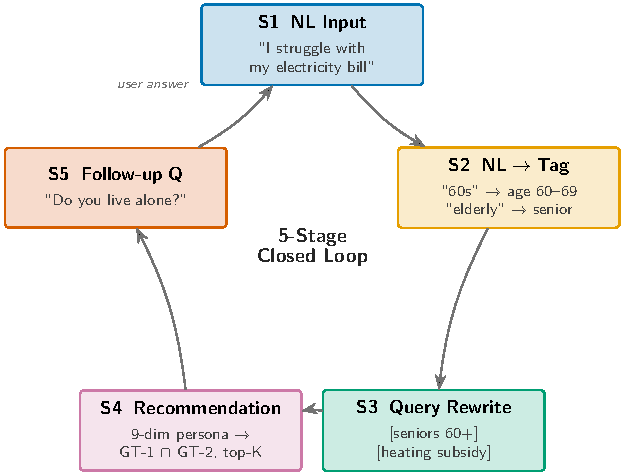
\includegraphics[width=\columnwidth]{figures/fig4_conv_loop.pdf}
\caption{Five-stage conversational loop. S1 receives a free-form
utterance (voice through STT or text); S2 updates a partial
9-dimensional persona vector (revealed/negated/unknown); S3 rewrites
the query conditioned on the partial vector; S4 retrieves
eligibility-aware candidates (rule prefilter $+$ dense rerank); S5
selects the next attribute to elicit. The user's reply re-enters S1.}
\label{fig:convloop}
\end{figure}

\textbf{S1 NL input.} Free-form utterance (voice or text).
\textbf{S2 NL$\to$tag extraction.} An LLM extractor maps the running
dialogue history to a partial 9-dimensional persona attribute vector
plus the free-text intent; each slot is \emph{revealed},
\emph{negated}, or \emph{unknown}.
\textbf{S3 Query rewriting.} The user's utterance is rewritten
conditioned on the partial attribute vector, expanding domain-elided
context (e.g., adding ``rent assistance'' when the user said
``\textit{my son's housing}'') and discarding tokens that duplicate
already-revealed attributes.
\textbf{S4 Eligibility-aware recommendation.} The current attribute
vector restricts the GT-1 candidate set, the rewritten query
restricts the GT-2 candidate set, and the rule $+$ dense rerank of
\S\ref{sec:exp} produces a ranked top-$K$.
\textbf{S5 Follow-up question.} The system selects the next attribute
to elicit from among the still-unknown slots and surfaces it as a
natural-language question.

\subsection{Evaluation Scope, Soft Eligibility, Selector}
\label{sec:conv:scope}

\textbf{Scope.} Stages S2--S3 are deployed but not benchmarked here:
\kwbench{} governs S4 (eligibility-aware retrieval) and S5
(follow-up selection). We evaluate the architecture as
\emph{progressive attribute revelation}: at each turn the system
invokes S5 to select an attribute, and an oracle reveals its true
value, simulating a successful S1--S3 loop.
\textbf{Soft eligibility.}
We replace the hard eligibility predicate with a \emph{soft}
score: revealed attributes contribute hard $\{0,1\}$, unrevealed
attributes contribute the corpus marginal $\hat{P}_t$. Full
equations in Appendix~\ref{app:soft_elig}.
\paragraph{Trained selector positioning.}
As a simpler counterpart to
\textsc{CLARINET}~\citep{andukuri2024clarinet}, we train a
\texttt{RandomForest} ($n{=}200$, depth 10) on 29-dim features
over an 80/20 persona-level split (144/36); both $\hat{P}_t$ and
the selector are estimated only on the 144 training personas.
Hyperparameter detail in Appendix~\ref{app:repro}.

\paragraph{LOPO robustness check.}
Leave-one-persona-out CV on the 144 training personas yields
turn-5 Recall@10 $= 0.090$ [$0.085, 0.094$] for trained vs.\
$0.074$ [$0.069, 0.078$] heuristic (paired bootstrap $+0.016$,
significant), tracking the leak-free $0.095$ closely; per-fold
detail in Appendix~\ref{app:lopo}.

\paragraph{Simpler clarification baselines.}
The most informative comparator is $\epsilon$-greedy
($\epsilon{=}0.1$) over attribute information-gain (IG), which
requires no learned model. On the 36 leak-free test personas at
turn~5 the trained selector reaches $0.095$ [$0.088$, $0.103$] and
$\epsilon$-greedy(IG) reaches $0.092$ [$0.084$, $0.100$] (paired
diff $+0.003$ [$-0.004$, $+0.011$], n.s.); heuristic $0.071$, random
$0.050$, oracle $0.103$. We therefore position the trained selector
not as a methodological contribution but as a
deployment-feasibility demonstration: when $\epsilon$-greedy(IG)
already matches accuracy, the operational question is inference
cost, where the RandomForest's ${\sim}1$\,ms predict beats IG's
${\sim}60$\,ms (10 dense reranks) per turn---more than an order of
magnitude. A Thompson-sampling baseline and
the CLARINET head-to-head are deferred to
Appendix~\ref{app:thompson} and future work, respectively.

\subsection{Results: Trained ML vs.\ IG vs.\ Heuristic vs.\ Oracle}
\label{sec:conv:result}

We compare four selectors over turns 0--5 with identical retrieval
(soft eligibility plus dense rerank, \S\ref{sec:conv:scope}):
\textbf{Heuristic} (fixed priority list, no learning),
\textbf{IG dynamic} (exhaustive per-turn IG trial, no learning),
\textbf{Trained ML} (the RandomForest above), and \textbf{Oracle}
(lookup of the actually best attribute at training time).

\begin{table}[t]
\centering\footnotesize
\setlength{\tabcolsep}{3pt}
\renewcommand{\arraystretch}{1.08}
\begin{tabular}{c@{\hspace{5pt}}rrrr}
\toprule
Turn & Heuristic & IG dyn. & \textbf{Trained ML} & Oracle \\
\midrule
0 & 0.003\,{\tiny[.002,.005]} & 0.003\,{\tiny[.002,.005]} & 0.003\,{\tiny[.002,.005]} & 0.003\,{\tiny[.002,.005]} \\
1 & 0.001\,{\tiny[.000,.003]} & 0.059\,{\tiny[.050,.067]} & \textbf{0.060}\,{\tiny[.051,.069]} & 0.063\,{\tiny[.055,.071]} \\
2 & 0.009\,{\tiny[.006,.012]} & 0.087\,{\tiny[.081,.094]} & 0.084\,{\tiny[.077,.091]} & 0.090\,{\tiny[.083,.097]} \\
3 & 0.073\,{\tiny[.066,.080]} & 0.091\,{\tiny[.085,.098]} & 0.090\,{\tiny[.083,.097]} & 0.098\,{\tiny[.091,.106]} \\
4 & 0.071\,{\tiny[.063,.080]} & 0.090\,{\tiny[.084,.096]} & 0.096\,{\tiny[.089,.103]} & 0.102\,{\tiny[.095,.110]} \\
5 & 0.071\,{\tiny[.062,.080]} & 0.095\,{\tiny[.087,.102]} & 0.095\,{\tiny[.088,.103]} & 0.102\,{\tiny[.095,.111]} \\
\bottomrule
\end{tabular}
\caption{Recall@10 over turns on $n{=}36$ leak-free test personas
(bootstrap mean and 95\% CI in brackets,
$N_{\mathrm{boot}}{=}10{,}000$). Trained ML and IG both beat the
Heuristic from turn~1 onward (paired Wilcoxon $p{<}10^{-4}$).
Trained ML and IG are not statistically distinguishable in accuracy
at any turn ($p\in[0.22,0.88]$); the differential is inference
cost.}
\label{tab:conv}
\end{table}

\paragraph{Inference-cost win.}
\label{sec:conv:cost}
IG dynamic must simulate soft scoring and dense reranking for every
candidate attribute (up to ten) at every turn---roughly ten retrieval
calls per persona-turn, each over \npolicy{} policies. The Trained ML
selector instead requires a single \texttt{predict\_proba} call
($\sim{}1$\,ms). When IG and ML are statistically tied on accuracy
(Table~\ref{tab:conv}), ML wins on user-facing latency, the
operational constraint of any deployed dialogue system. At turn~5
both reach roughly $93\%$ of the oracle ceiling
($0.0953/0.0950$ vs.\ $0.1025$).

\paragraph{Narrowing the access gap.}
Trained ML at turn~5 ($0.0953$) is roughly an order of magnitude
above the single-shot BM25 query-only baseline ($0.0071$, 180
personas, eligibility-blind); the two settings differ on multi-turn
vs.\ single-shot, eligibility-aware vs.\ blind, and $n{=}36$ vs.\
180, so the figure quantifies the joint architecture benefit, not
the marginal selector contribution. The matched-$n{=}36$ selector
gap is trained$-$heuristic $+0.025$ at turn~5
(Table~\ref{tab:conv}, paired bootstrap
significant).

% =====================================================================
\section{Limitations}
\label{sec:limit}

L1--L6 bound the \emph{benchmark}; L7--L12 bound the
\emph{architectures}. \textbf{(L1)} Eligibility conditions outside
the \ndim{}-binary $+$ 3-numeric schema are absent by construction.
\textbf{(L2)} April~2026 snapshot; policy drift and seasonal
programs are not measured. \textbf{(L3)} Sub-regional preferences
in PDF/HWP attachments are partially recovered by the GT-2 free-text
channel but absent from GT-1. \textbf{(L4)} Sub-municipal regions
(\texttt{dong}, \texttt{eup}, \texttt{myeon}) are not represented.
\textbf{(L5)} \npersona{} personas cover five reference groups and
18 compound axes; some intersectional cells (e.g.\ rural
single-parent foreign-born) have single-digit counts. The generator
is shipped seed-pinned for community-extensible expansion targeting
$1{,}000{+}$ personas. \textbf{(L6)} Reviewers behind every
disagreement-adjudication are graduate students and domain
practitioners, not licensed social workers; their output is a strong
tier above pure LLM labels but below a formal expert audit.

\textbf{(L7)} GT-2 labels are produced by LLM-as-judge at
temperature~0; cross-LLM agreement is $\kappa_w{=}0.69$, and residual
judge bias correlated across the two vendors cannot be fully excluded
by cross-vendor agreement alone. \textbf{(L8)} The query pool assumes the
user is the prospective beneficiary; family-proxy search is out of
scope. \textbf{(L9)} Two query phrasings per sub-topic; paraphrase
robustness and spoken disfluencies are absorbed upstream by the
conversational architecture, not stress-tested at the pool level.
\textbf{(L10)} The 80/20 conversational split is in-distribution;
the $1{,}000{+}$-persona L5 expansion is the planned OOD route.
\textbf{(L11)} STT error and upstream NL-stage mismatch are not
quantified here; a controlled user study with eligibility-recovery
scores is in progress. \textbf{(L12)} Calibrated for the Korean
Bokjiro taxonomy; cross-jurisdiction transfer requires a
sub-topic discovery pass.

% =====================================================================
\section{Conclusion and Social Impact}
\label{sec:conclusion}\label{sec:ethics}

\kwbench{} is a cell-level Korean welfare evaluation resource
(\npolicy{} policies, \npersona{} personas, \ndim{}-binary schema,
66-query pool, three ground-truth tables). Korean-domain dense
retrieval is the strongest rule-free baseline on GT-2 (NDCG@10
$0.86$, $p{<}10^{-8}$ over BM25); no rule-free retriever exceeds
NDCG@10 $0.13$ on GT-3-strict; under a matched rule prefilter,
dense rerank beats Gemini LLM rerank by $+0.46$. A 1\,ms
RandomForest selector statistically matches exhaustive IG on
Recall@10 (turn-5 difference $\leq{}0.3\%$, n.s.) at ${\sim}60\times$
less inference. Risks are mitigated by surfacing
matches as \emph{candidates} (agency-confirmed) and by two-LLM
full pass plus human adjudication on every LLM-judged layer;
personas are synthetic (no PII). Future work: $1{,}000{+}$-persona
expansion, credentialed-expert audit, trained NL$\to$tag at S2,
and real-user evaluation of S1--S3.

% =====================================================================
\section*{Acknowledgements}

This research was supported by the MSIT (Ministry of Science and ICT),
Korea, under the ITRC (Information Technology Research Center) support
program (IITP-2026-RS-2020-II201789), and the Artificial Intelligence
Convergence Innovation Human Resources Development
(IITP-2026-RS-2023-00254592) supervised by the IITP (Institute for
Information \& Communications Technology Planning \& Evaluation).

% =====================================================================
\clearpage
\bibliographystyle{icml2026}
\bibliography{refs}

% =====================================================================
\clearpage
\appendix
\onecolumn

\section{Full Tag Schema}
\label{app:schema}

The \kwbench{} labeling schema groups \ndim{} binary tags under five
top-level macro-categories together with three numeric fields. Each
binary tag takes one of three values: $-1$ \emph{excluded}
(disqualifies the applicant), $0$ \emph{indifferent} (not mentioned),
$+1$ \emph{required}. The same vocabulary is used on both the policy
side (A3) and the persona side (A5), so the GT-1 eligibility function
operates on a single shared schema.

\subsection*{A.1 Binary Tag Inventory}

\begin{itemize}[leftmargin=*]
\item \textbf{PERSONAL (14 binary).}
  \begin{itemize}[leftmargin=*,nosep]
  \item \texttt{personal.gender (2)} --- female\_only, male\_only.
  \item \texttt{personal.disability (5)} --- required\_any, severe,
        developmental, visual, hearing.
  \item \texttt{personal.health (7)} --- chronic\_or\_severe,
        rare\_or\_cancer, mental\_health, dementia, diabetes,
        hypertension, depression.
  \end{itemize}

\item \textbf{ECONOMIC (14 binary).}
  \begin{itemize}[leftmargin=*,nosep]
  \item \texttt{economic.income (3)} --- basic\_recipient,
        secondary, medical\_aid.
  \item \texttt{economic.employment (7)} --- unemployed,
        self\_employed, startup, agriculture\_fishery,
        small\_business\_sme, public\_servant\_military,
        industrial\_accident.
  \item \texttt{economic.housing (4)} --- no\_house, jeonse,
        monthly\_rent, rental.
  \end{itemize}

\item \textbf{HOUSEHOLD (14 binary).}
  \begin{itemize}[leftmargin=*,nosep]
  \item \texttt{household.type (7)} --- single, single\_parent,
        multi\_child, newlywed, multicultural, grandparent,
        youth\_minor.
  \item \texttt{household.pregnancy (4)} --- pregnant\_postpartum,
        infertility, unmarried\_mother, birth.
  \item \texttt{household.birth\_order (3)} --- first, second,
        third\_plus.
  \end{itemize}

\item \textbf{SOCIAL (20 binary).}
  \begin{itemize}[leftmargin=*,nosep]
  \item \texttt{social.veteran (4)} --- war\_veteran,
        national\_merit, independence, veteran\_family.
  \item \texttt{social.immigrant (3)} --- foreigner\_general,
        north\_korean\_defector, late\_arrival\_child.
  \item \texttt{social.vulnerable (6)} --- vulnerable\_general,
        crisis\_household, homeless, solo\_elderly,
        foster\_or\_protected\_child, adoption.
  \item \texttt{social.violence\_victim (1)} --- violence.
  \item \texttt{social.education (4)} --- elementary\_to\_high,
        university, out\_of\_school, ged.
  \item \texttt{social.residence (2)} --- resident\_required,
        long\_term\_resident.
  \end{itemize}

\item \textbf{POLICY (7 binary).}
  \begin{itemize}[leftmargin=*,nosep]
  \item \texttt{policy.category (7)} --- welfare, employment,
        education, housing, health, culture, living. Inherits the
        seven Bokjiro operational categories.
  \end{itemize}
\end{itemize}

\subsection*{A.2 Numeric Fields (3)}

\begin{itemize}[leftmargin=*,nosep]
\item \texttt{age\_min} (\texttt{int|null}) --- lower bound;
      \texttt{null} when no lower bound is stated.
\item \texttt{age\_max} (\texttt{int|null}) --- upper bound;
      \texttt{null} when no upper bound is stated.
\item \texttt{median\_threshold} (\texttt{int|null}) --- percentage
      of national median income required for eligibility;
      \texttt{null} when no income threshold is stated.
\end{itemize}

All three numeric fields are populated only when explicitly stated
by the policy text.

\subsection*{A.3 Schema Example: Policy and Persona Tagging}

To illustrate how a single schema is shared between the policy and
persona sides of GT-1, we walk through one (policy, persona) cell.

\paragraph{Policy: ``Seoul Youth Monthly Rent Support''.}
The encoded \texttt{tag\_values} (showing only nonzero slots) are:
\begin{itemize}[leftmargin=*,nosep]
\item \texttt{personal.gender}: all $0$ (gender-indifferent).
\item \texttt{economic.income.basic\_recipient}{=}$+1$ (required:
      basic-recipient or secondary status).
\item \texttt{economic.income.secondary}{=}$+1$ (required).
\item \texttt{economic.housing.no\_house}{=}$+1$ (required: no
      ownership).
\item \texttt{household.type.single}{=}$+1$ (required: single-person
      household).
\item \texttt{social.residence.resident\_required}{=}$+1$ (required:
      registered Seoul resident).
\item \texttt{policy.category.housing}{=}$+1$.
\item \texttt{age\_min}{=}19, \texttt{age\_max}{=}39,
      \texttt{median\_threshold}{=}150 (i.e.\ $\leq{}150\%$ median).
\end{itemize}

\paragraph{Persona P\_YOU\_03 (Youth group).}
Synthetic \texttt{tag\_values}: age=24, gender=female, sido=``Seoul'',
sigungu=``Gwanak-gu'', \texttt{economic.income.secondary}{=}$+1$
(satisfied), \texttt{economic.housing.no\_house}{=}$+1$ (satisfied),
\texttt{household.type.single}{=}$+1$ (satisfied),
\texttt{social.residence.resident\_required}{=}$+1$ (satisfied),
median\_income\_pct=120.

\paragraph{GT-1 cell evaluation.}
The deterministic eligibility function checks all nine dimensions
(\S\ref{sec:bench:a7}): age $19\leq{}24\leq{}39$ \checkmark; income
secondary required and persona has secondary status \checkmark;
\texttt{no\_house} required and persona satisfies \checkmark;
\texttt{single} household required and persona satisfies \checkmark;
Seoul residency required and persona is in Gwanak-gu (Seoul)
\checkmark; median threshold $150$ and persona at $120$ \checkmark.
Result: \texttt{eligible(P\_YOU\_03, this policy)}{=}$1$.

\paragraph{GT-2 cell evaluation.}
Independently, query Q$_{17}$ (``\textit{rent is becoming hard to
afford}'', a persona-orthogonal situational phrasing under R1) is
graded by the LLM judge against this policy. Both
\texttt{gpt-5.4-nano} and \texttt{gemini-2.5-flash-lite} return
grade $=2$ (direct topical match), so this (query, policy) cell is
in GT-2 at the strict threshold.

\paragraph{GT-3 cell.}
Since GT-1$=1$ \emph{and} GT-2$\geq{}2$ \emph{and} the strict region
predicate matches (persona Seoul, policy Seoul), this (persona, query,
policy) triple lies in GT-3-strict.

\section{Baseline Pseudocode}
\label{app:baselines}

\subsection{B1 BM25}
\begin{verbatim}
def tokenize(text):
    # Korean word tokens + 2-gram syllable backoff
    words = re.split(KOREAN_WORD_BREAK, text)
    tokens = []
    for w in words if len(w) >= 2:
        tokens.append(w)
        for i in range(len(w) - 1):
            tokens.append(w[i:i+2])
    return tokens

def fit(policies):
    return BM25Okapi([tokenize(policy_text(p)) for p in policies])

def retrieve(persona, k):
    q = tokenize(persona.query + persona.attribute_keywords)
    return top_k_by_score(policy_ids, bm25.get_scores(q), k)
\end{verbatim}

\subsection{B2 Dense Embedding}
Model: \texttt{jhgan/ko-sroberta-multitask} (768-d Korean SBERT).
Policy text and persona query are encoded and ranked by L2-normalized
cosine similarity.

\subsection{B3 Hybrid (Reciprocal Rank Fusion)}
\[
\mathrm{score}_{\text{hybrid}}(p) =
\frac{1}{k_{\text{rrf}} + r_{\text{BM25}}(p)}
+ \frac{1}{k_{\text{rrf}} + r_{\text{dense}}(p)},
\quad k_{\text{rrf}}{=}60.
\]
Each retriever contributes its top $\max(K{\times}5, 100)$
candidates.

\subsection{B4 Graph (Tag Overlap)}
Let $R(p) = \{t : \text{label}(p,t) = +1\}$ and $S(\pi)$ be persona
$\pi$'s satisfied-tag set; the score is
$|R(p)\cap S(\pi)|/\sqrt{|R(p)|\cdot|S(\pi)|}$.

\subsection{B5 LLM-rerank}
BM25 prefilters 50 candidates; \texttt{gemini-2.5-flash-lite}
receives the persona context and the candidate list and returns
top-$K$ identifiers in comma-separated form with structured-output
enforcement.

\subsection{B6 Rule $+$ Dense rerank}
\begin{enumerate}[leftmargin=*,nosep]
\item Apply the rule eligibility function to obtain the candidate
set (mean 97 policies).
\item Score each candidate's dense embedding against the persona
query embedding (cosine).
\item Return the top-$K$.
\end{enumerate}
B2$+$rule is by construction identical to B6 (different naming
emphasizes the matched-prefilter perspective in
Table~\ref{tab:gt3}).

\section{Soft Eligibility Scoring}
\label{app:soft_elig}

For persona $\pi$, policy $q$, revealed attribute set
$R \subseteq \mathcal{A}$:
\[
\mathrm{score}(\pi, q; R) = \sum_{t \in T_q} \log \tilde{P}_t(\pi, q; R),
\]
where $T_q = \{t : \text{label}(q,t) \neq 0\}$ and
\[
\tilde{P}_t = \begin{cases}
P_t(\pi) & \text{if } a(t) \in R \text{ (hard match, } \in\{0,1\}) \\
\hat{P}_t & \text{if } a(t) \notin R \text{ (marginal estimate)}
\end{cases}
\]
$a(t)$ is the persona attribute on which tag $t$ depends. When
$\text{label}(q,t)=-1$, we substitute $1-\tilde{P}_t$. To avoid
$\log 0$ we clip to $[10^{-6}, 1.0]$. The marginal $\hat{P}_t$ is
estimated on the 144 training personas:
$\hat{P}_t = N_{\text{train}}^{-1} \sum_{\pi}
\mathbb{1}[\pi \text{ satisfies } t]$.
For numeric and region tags: when revealed, $\log(10^{-6})$ is
added on mismatch (effective disqualification); when unrevealed,
the marginal is used.

\section{Persona Examples, Reproducibility, and Auxiliary Results}
\label{app:persona}\label{app:repro}

\paragraph{Persona examples.}
\textbf{P\_DIS\_01 (Disability group):} age 65, male, Seoul
Seodaemun-gu, secondary income, present disability, employed; query
``\textit{Can my disabled child receive education-fee support?}''
\textbf{P\_INT\_15 (Intersectional):} age 73, female, Busan
Haeundae-gu, basic-recipient income, present disability,
single-person household, special target solo elderly.
\textbf{P\_GEN\_22 (General):} age 35, male, Gyeonggi Suwon, general
income, no disability, newlywed household, employed.

\paragraph{A3 tagging cost.}
We ran the A3 tag-extraction prompt against \texttt{gpt-5.4}
(April~2026, temperature~0) with 16 concurrent workers; the full
\npolicy{}-policy pass completed in roughly 13 minutes. The
comma-separated output format reduces output tokens
$790\to{}144$ per policy on average ($5.5{\times}$); total cost is
approximately \$23 for the full corpus.

\paragraph{Index build.}
BM25 index build is 0.41\,s on a single CPU; dense and hybrid
indices build in 9.93\,s and 10.34\,s respectively.

\paragraph{Auxiliary results.}
\label{app:auxiliary}\label{app:lopo}\label{app:thompson}%
\textbf{ko-reranker:} \texttt{Dongjin-kr/ko-reranker} reranks BM25
top-200, NDCG@10 $0.803$ (below BGE-reranker-v2-m3 $0.853$ and BGE-M3
$0.815$). \textbf{LOPO per-fold:} held-out per-persona Recall@10
trained $0.090$ [$0.085, 0.094$] vs.\ heuristic $0.074$
[$0.069, 0.078$], paired trained--heuristic $+0.016$
[$+0.013, +0.020$]; per-fold dispersion released with result tables.
\textbf{Thompson sampling:} Beta(1,1) prior per attribute, updated
with observed IG. At the 5-turn budget the policy under-explores
($0.049$ [$0.037, 0.061$], numerically below random $0.050$). The
failure is a horizon/prior mismatch: with an uninformative Beta(1,1)
prior and only five updates the posterior over per-attribute
information gain stays near-flat, so draws are effectively uniform and
the short turn budget leaves no room to recover from an unlucky early
pull; the net behavior approximates random selection. An informative
prior or a longer horizon would be required for Thompson sampling to
become competitive with $\epsilon$-greedy(IG).

\end{document}
